\documentclass{article}
\usepackage[utf8]{inputenc}
\usepackage{amstext}
\usepackage{amsmath} 
\usepackage{mathpazo}
\usepackage{graphicx} 
\usepackage{float} 
\usepackage{caption} 
\usepackage{epstopdf} 
\usepackage{hyperref}
\usepackage{varioref} 
\usepackage{fancyref}
\usepackage[section]{placeins} 
\usepackage{perpage}
\usepackage[margin=1in, paperwidth=8.5in, paperheight=11in]{geometry} 
\MakeSorted{figure} 
\usepackage{natbib}
\usepackage{graphicx}
\usepackage{xcolor}
\usepackage{listings}
\usepackage{minted}
\usepackage{subcaption}
\usepackage{eso-pic}
\usepackage{tikz}
\usepackage[american]{circuitikz}
\usepackage[font=small,labelfont=bf]{caption}

\title{ENGR2420 Lab 9 : Current-Mirror Differential Amplifier}
\author{Abigail Fry\\ Anusha Datar\\ Vienna Scheyer}
\date{April 29, 2019}

\begin{document}

\maketitle
\section{Experiment One : Voltage Transfer Characteristics}
In this experiment, we constructed a current-mirror differential amplifier with an nMOS differential pair, two pMOS current mirrors, and an nMOS current mirror. We set the bias voltage to $0.69$ Volts so that the bias current was on the order of microamps. We then connected the inverting input, $V_2$, to $2, 3,$ and $4$ Volts and swept the value of the noninverting input while measuring the voltage output. 

\begin{figure}[H]
  \begin{center}      
  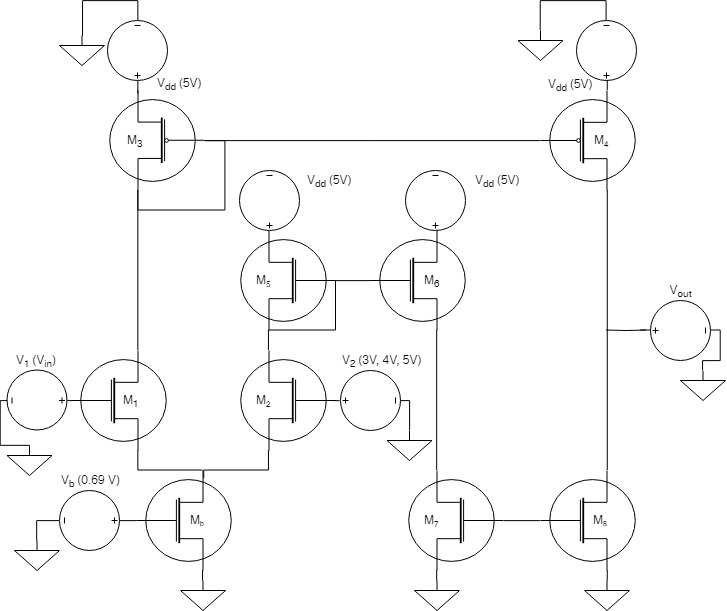
\includegraphics[scale = 0.5]{images/exp1_schematic.jpg}
  \caption{Schematic of circuit characterized in experiment one.}   
  \label{fig:exp1_schematic}
  \end{center}
\end{figure}

\subsection{Results}
We collected voltage transfer characteristics for the differential amplifier with the value of $V_2$ set to 2, 3, and 4 Volts and with $V_b$ set to 0.69 Volts so that our bias transistor was in moderate inversion. 
\begin{figure}[H]
  \begin{center}      
  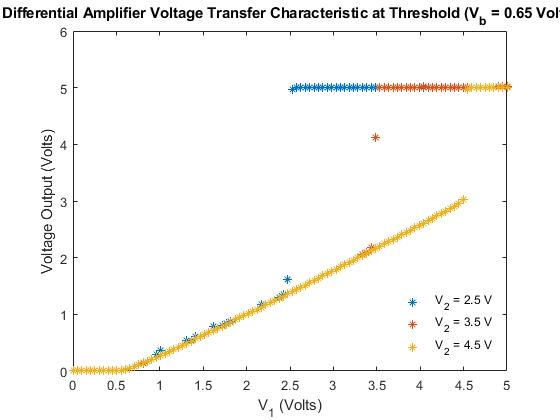
\includegraphics[scale = 0.3]{images/exp1_plot1.jpg}
  \caption{Current-Mirror Differential Amplifier voltage transfer characteristic.}   
  \label{fig:exp1_plot1}
  \end{center}
\end{figure}

\subsection{Analysis}
We expected the voltage transfer characteristic to rail towards ground when $V_1 < V_2$ and then quickly swing from ground to $V_{dd}$ when $V_2 > V_1$. At the instant where $V_1 = V_2$, the voltage quickly shifts. Our experimental data closely reflects this pattern at all three voltages as seen in Figure \ref{fig:exp1_plot1}.

\subsection{Discussion}
This differential amplifier has much more dramatic rail-to-rail output swing than the simple differential amplifier studied in Lab 8. The transition region is nearly nonexistent - the voltage quickly shifts from ground to $V_{dd}$.

\section{Experiment Two : Transconductance, Output Resistance, and Gain}

In this experiment, we varied the differential-mode voltage of the inputs and measured the output voltage to extract the differential-mode gain of the circuit.  Next, we measured the output current and output voltage to extract the incremental output resistance of the circuit.  Finally, we swept the differential-mode voltage and plotted the output current to extract the incremental transconductance gain.  To collect this data, we set $V_{b} = 0.69$ Volts and while finding the output resistance we also set $V_{2} = 3$ Volts. We used the schematic seen in Figure \ref{fig:exp2_schematic}.
\begin{figure}[H]
  \begin{center}      
  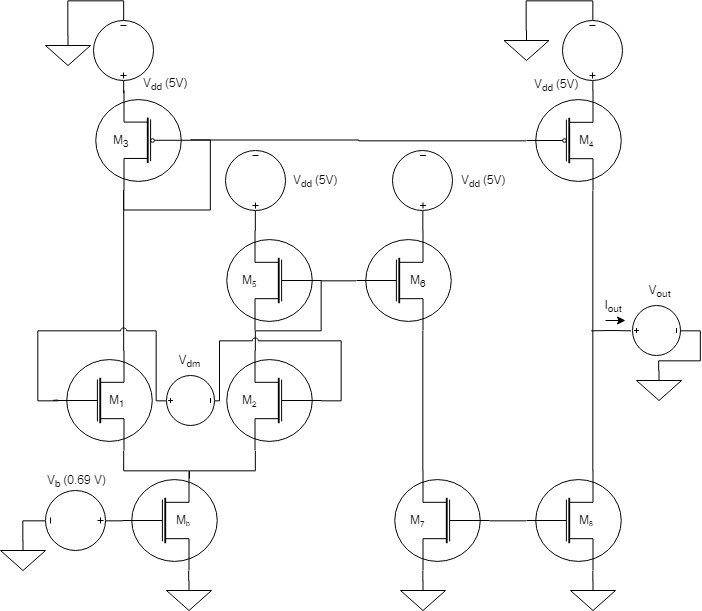
\includegraphics[scale = 0.5]{images/exp2_schematic.jpg}
  \caption{Schematic for Experiment 2}   
  \label{fig:exp2_schematic}
  \end{center}
\end{figure}

\subsection{Results}
First, we plotted the differential-mode voltage vs. the output voltage on linear axes.  We found $A_{dm}$ by fitting a line to the steep part of the curve and extracting the slope of that region.  The differential-mode gain for the plot in Figure \ref{fig:DGM} is $A_{dm} = 165.1419$.  Differential-mode gain does not have units because it is a ratio of voltages.

\begin{figure}[H]
  \begin{center}      
  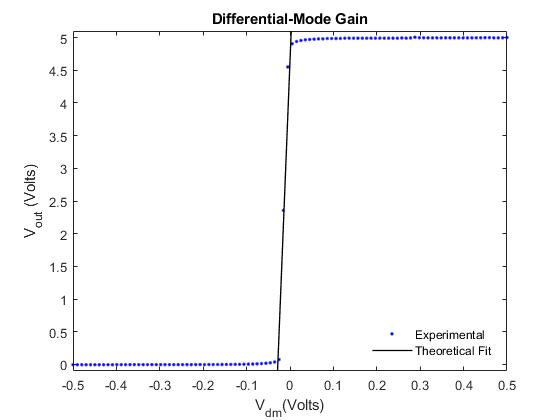
\includegraphics[scale = 0.5]{images/2_DGM.jpg}
  \caption{Output voltage vs. differential-mode voltage for the current mirror differential amplifier}   
  \label{fig:DGM}
  \end{center}
\end{figure}

Next, we plotted the output current vs. output voltage on linear axes.  We found the output resistance, $R_{out}$, by fitting a line to the shallow part of the curve using $polyfit$ and taking the inverse of the slope of the line.  The output resistance for the plot in Figure \ref{fig:OR} is $R_{out} = 9.1428 M \Omega$.

\begin{figure}[H]
  \begin{center}      
  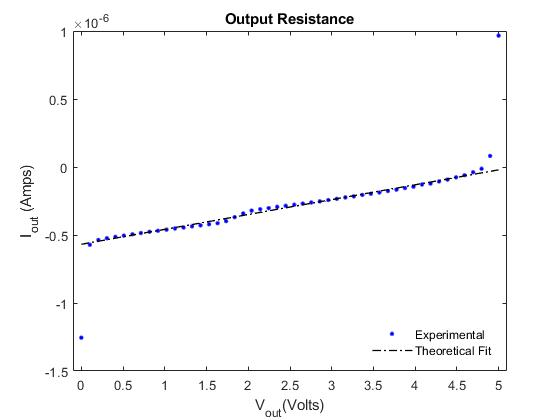
\includegraphics[scale = 0.5]{images/2_OR.jpg}
  \caption{Output voltage vs. output current for the current mirror differential amplifier}   
  \label{fig:OR}
  \end{center}
\end{figure}

Finally, we plotted the differential-mode voltage vs. the output current.  We found $G_{m}$ by fitting a straight line to where $V_{1} = V_{2}$ and extracting the slope.  The incremental transconductance gain of the plot in Figure \ref{fig:TG} is $G_{m} = 0.000020107$ mhos.

\begin{figure}[H]
  \begin{center}      
  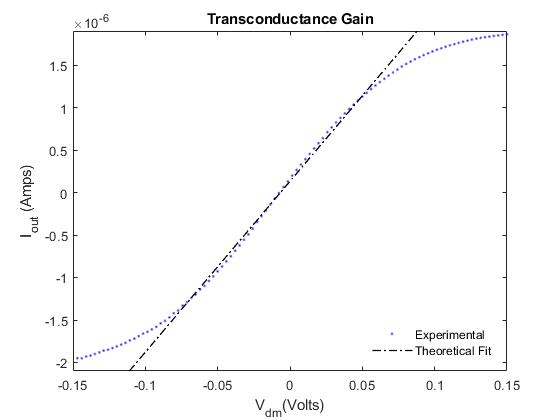
\includegraphics[scale = 0.5]{images/2_TG.jpg}
  \caption{Differential-mode voltage vs. output current for the current mirror differential amplifier}   
  \label{fig:TG}
  \end{center}
\end{figure}
\subsection{Analysis}
The equation for incremental differential-mode voltage gain of the circuit can be calculated using the equation below.
\begin{center}
 $A_{dm} = \frac{\delta V_{out}}{\delta V_{dm}} = \frac{\delta V_{out}}{\delta I_{out}} \times \frac{\delta I_{out}}{\delta V_{dm}} = R_{out} \times G_{m}$
   \end{center}
   
 By using the values we extracted in Figure \ref{fig:OR} and Figure \ref{fig:TG}, we were able to calculate the value of differential-mode voltage gain.  Then we compared it to the value extracted from Figure \ref{fig:DGM}.  The extracted value of $A_{dm}$ was 165.1419 and the value calculated was $A_{dm} = 183.8302$.  To quantify the difference between those values we used the percent error equation and found a $11.3 \%$ error between our theoretical (extracted) and experimental (calculated) values. 
 \begin{center}
Percent Error= $\frac{|(Theoretical-Experimental|}{Experimental}\times 100$ 
 \end{center}
\subsection{Discussion}

The percent error between the calculated value and extracted value of $A_{dm}$ for the data we collected was $11.3 \%$.  This percent error makes sense due to the way we extracted $R_{out}$ and $G_{m}$.  We used MATLAB's $polyfit$ function on specific parts of the curves in Figure \ref{fig:OR} and Figure \ref{fig:TG} to extract the values.  The range of data points used in the $polyfit$ function were qualitatively selected.   This means there is some level of error between experimental and theoretical $R_{out}$ and $G_{m}$.  This explains why the percent error between the calculated and extracted $A_{dm}$ is around $ 10 \%$.

The extracted value of $A_{dm}$ was 138.6165 for Lab 8, compared to ${A_{dm} = 165.1419}$ from this lab.  The simple MOS differential amplifier has a smaller gain than the current-mirror differential amplifier 
\section{Experiment Three : Differential Pair Current–Voltage Characteristics}
In the third experiment, we configured our amplifier as a unity-gain follower by connecting the output to the inverting input. We then loaded our follower-connected amplifier with a 1 nF capacitor connected between the output of our amplifier and ground.

Next, we applied both a small-amplitude (.050 V) and large-amplitude (2 V) square wave to the input of the circuit and observed both the input and output waveforms as a function of time. 
\begin{figure}[H]
  \begin{center}      
  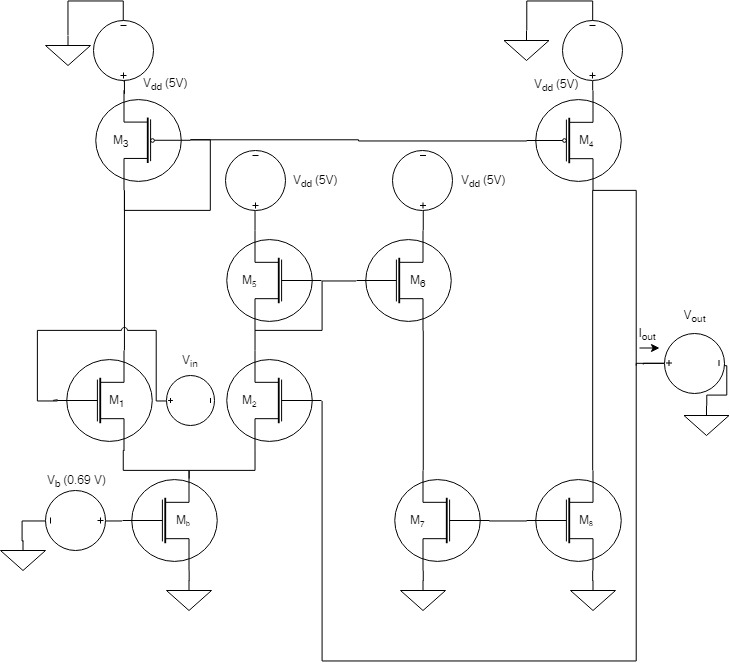
\includegraphics[scale = 0.5]{images/exp3_schematic.jpg}
  \caption{Experiment Three Schematic.}   
  \label{fig:exp1_schematic}
  \end{center}
\end{figure}

\subsection{Results}
We first studied the relationship between the input and output waveforms with a square wave input with an amplitude of $0.05$ Volts. 
\begin{figure}[H]
  \begin{center}      
  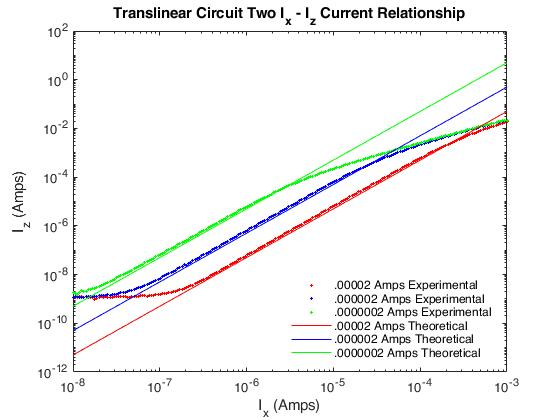
\includegraphics[scale = 0.2]{images/exp3_plot1.jpg}
  \caption{Unity gain follower dynamics with small-amplitude input.}   
  \label{fig:exp1_schematic}
  \end{center}
\end{figure}
We calculated the time constants for both the increasing and decreasing behaviors by using $polyfit$ on the log of the output voltage offset by the input voltage. The time constant for the increasing behavior is 3.5871e-05 seconds, and the time constant for the decreasing behavior is 2.4950e-05 seconds.

Then we performed the same operation with a square wave input of $2V$. Figure \ref{fig:slew_rate} shows the large-amplitude input unity gain follower behavior.

\begin{figure}[H]
  \begin{center}      
  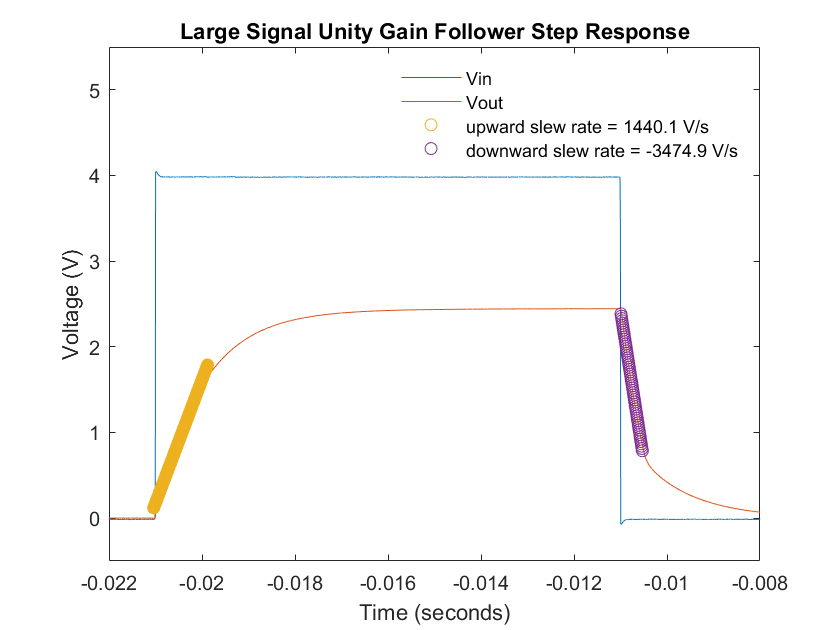
\includegraphics[scale = 0.5]{images/slew_rate.png}
  \caption{Unity gain follower dynamics with large-amplitude input.}   
  \label{fig:slew_rate}
  \end{center}
\end{figure}

We extracted the slew rates of the increasing and decreasing regions using the $polyfit$ function in MATLAB. The increasing region slew rate is 1440.1 $\frac{V}{s}$, and the decreasing region slew rate is -3474.9 $\frac{V}{s}$. 

\subsection{Analysis}
Theoretically, the output voltage of the unity-gain follower circuit should exactly match the input voltage. Experimentally, output roughly mirrors our input for the small amplitude case, even though there is a nontrivial delay in the transition region because it takes time for the capacitor to charge and discharge. 

For more rigorous analysis, we can calculate the RC time constant by calculating the rate at which $V_{out}$ changes as the capacitor charges and discharges. To do so, we used MATLAB's polyfit function on the logarithm of the times and the logarithm of $V_{out} - V{in} - \delta V{in}$ to extract the value of the slope. In doing so, we calculated that the time constant for the increasing behavior is 3.5871e-05 seconds, and the time constant for the decreasing behavior is 2.4950e-05 seconds.

We can also use $G_m$ to calculate the time constant. Because the time constant is equal to the product of resistance and capacitance, and $G_m$ is the reciprocal of the resistance, we can calculate the time constant with the equation $\frac{C}{G_m}$. In this case, the value of the time constant is $\frac{1e-09 Farads}{2.01e-05 Mhos}$ = 4.9751e-05 seconds. Ideally, both the increasing and decreasing behaviors should have this time constant. 

We can calculate the percent error by computing the quotient of the difference of the theoretical and experimental values and the experimental value. The percent error for the increasing behavior is $\frac{4.9751e-05 s - 3.5871e-05 s}{4.9751e-05}$ or 28.9 percent. The percent error for the decreasing behavior is $\frac{4.9751e-05 s - 2.4950e-05 s}{4.9751e-05}$ or 49.9 percent. While this is a nontrivial difference, there is also a great deal of variability associated with how we calculated these values (i.e. which points we chose to base our fits on, measurement errors, etc.) so it is within a reasonable range since they are within a similar order of magnitude. 

We calculated the expected maximum slew rate by taking the limiting value of the output current divided by the load capacitance. For the limiting value of the output current, we used $I_b = 10uA$ because earlier in the lab we chose $V_b$ such that $I_b$ would be on the order of microamps. The capacitance of the capacitor is $1nF$. Thus, the maximum expected slew rate would be $10000 \frac{V}{s}$.

\subsection{Discussion}
For the small-amplitude input, the response mirrors the behavior of the input square wave. But, they are not quite symmetrical, as it takes time for the capacitor to charge and discharge. In that way, it is a linear system - the output is proportional to the input, but there is some finite lag in the time domain. While the actual time constant has a nontrivial percent error, this is not surprising due to the amount of subjectivity in calculating the constants, and it is encouraging that they are on the same order of magnitude.  

For the large-amplitude input, the slew rates in the increasing and decreasing regions are not equivalent which is worth noting. Additionally, our experimentally extracted slew rates are less than $10000 \frac{V}{s}$, which is reasonable because our extracted slew rates are less than the expected maximum.

\end{document}
